\documentclass[11pt]{article}
%Gummi|065|=)
\title{\textbf{Annealing code \texttt{minAone} User Guide}}
\author{Jingxin Ye}
\date{\today}
\usepackage{graphicx}
\usepackage[numbers]{natbib}
\usepackage{graphicx}
\usepackage{subfigure}
\usepackage{amsmath}
\usepackage{verbatim}
\usepackage{multicol}
\usepackage[title]{appendix}
\usepackage[latin1]{inputenc}
\usepackage{tikz} 
\usetikzlibrary{matrix}
\usepackage{circuitikz}
\usepackage[normalem]{ulem}
\usepackage{mdframed}
\usepackage{hyperref}
\begin{document}

\maketitle
\tableofcontents
\newpage
\section{About \texttt{minAone}}
The annealing code \texttt{minAone} described in this document is used for calculating action levels of dynamical systems. The code is developed as an extention of \texttt{minAzero} written by Bryan Toth and Chris Knowlton. That is where the name \texttt{minAone} comes from. In another aspect, following the lowest action level $A_0$, $A_1$ represents the second lowest one, which is an interesting quantity we care about and has significant application in statistical data assimilation.
\section{Problem Statement}
Given a dynamical system modeled by $D$-dimensional discrete map
\[{x_a}(n+1)=f_a(\mathbf{x}(n)),~~a=1,\dots,D\]
the probability distribution of its states can be expressed as $P(X|Y)=\exp(-A_0)$, when $L$-dimensional obersations $Y$ are present.  If one assumes both measurement noises and model error are independent and gaussian, the action $A_0$ has the format of
\begin{align}
A_0(X) = &\sum_{n=0}^m\, \frac{R_m(n)}{2} \sum_{l=1}^L [x_l(n) - y_l(n)]^2 +  \frac{R_f}{2} \sum_{n=0}^{m-1} \sum_{a=1}^D[x_a(n+1) - f_a(\mathbf{x}(n))]^2 .
\label{eq:actionform}
\end{align}
where $R_m$ and $R_f$ are the inverse of variances.

The annealing method is based on the observation that the minima solution $X^q$ of $A_0$ at $R_f=0$ is $x_l(n)=y_l(n)$, the other $D-L$ components of the model state vector are undetermined, and the solution is degenerate. As we increase $R_f$, the action levels split, and depending on $R_m$, $R_f$, $L$ and the precise form of the dynamical vector field $\mathbf{f}(\mathbf{x})$, there will be 1,2,\dots minima of $A_0$.

\section{Annealing Procedure}
The annealing process proceeds as follows: with very small initial $R_f$, we call it $R_{f0}$, solve the $(m+1)D$-dimensional search problem with an optimization algorithm that seeks minima of $A_0(X)$. Start the search with a set of trial paths whose components are selected from a uniform distribution within limits suggested by examining the times series generated by the model $\mathbf{x} \to \mathbf{f}(\mathbf{x})$ (or any other selection process for the initial guess). This will generate a collection of approximate paths $X^q$. Increase $R_f$ by a small increment (we choose $R_f = \{R_{f0}\alpha^{\beta}\}$, where $\alpha=2, \beta = 0,1,\dots$ in our examples),  and using the paths found for the smaller $R_f$ as initial guesses, find a new set of approximate $X^q$. Continue this process until the lowest action level path $X^0$ produces a $A_0(X^0)$ near expected value, which can be identified from our knowledge of measurement noises. In our example, as the values $[y_l(n) - x_l(n)]\sim\mathcal{N}(0,\sigma^2)$ by our choice, the measurement error term  $\sum_{n=0}^m \sum_{l=1}^L [(x_l(n) - y_l(n))/\sigma]^2/2$ has a $\chi^2$ distribution with $L(m+1)$ degrees of freedom. The mean and uncertainty of this distribution over different choices of noise waveforms are $(m+1)L/2$ and $\sqrt{(m+1)L/2}$, respectively.

After identifying the global minima and other local minima of $A_0$, we can employ laplace method to approximate the expected value $\langle G(X) \rangle$ of a function $G(X)$ is 
\begin{equation}
\langle G({X}) \rangle = \frac{\int dX\, G(X) \exp[-A_0(X)]}{\int dX\, \exp[-A_0(X)]}\approx G(X^0).
\label{eq:expect}
\end{equation}
plus exponentially small corrections.
If the action level $A_0(X^0)$ is substantially less than the action level on the next path $A_0(X^0) \ll A_0(X^1)$, all statistical data assimilation expected values $\langle G(X)\rangle$ are given by $X^0$ and fluctuations about that path with exponential accuracy of order $\exp[-(A_0(X^1) - A_0(X^0))]$.
\section{Installing Required Programs and Packages}
This document will assume that the user is using a Linux distribution and has basic compliers installed including gcc, gfortran and python.
\subsection{Python Packages}
These python scripts link to the sympy library.  To install these, use \texttt{apt-get/yum install sympy} or download directly from sympy.org.
\subsection{IPOPT}
\subsubsection*{Download}
Get it here: \url{https://projects.coin-or.org/Ipopt}
\begin{itemize}
\item Download and unzip latest version of IPOPT 
\item As of right now this is 3.11.7 - Efficacy of installation instructions may degrade over time as packages are updated.
\item Go into ThirdParty folder in the IPOPT directory then do the following commands.
\end{itemize}
\begin{verbatim}
$ cd Blas
$ ./get.Blas
$ cd ../Lapack
$ ./get.Lapack
$ cd ../ASL
$ ./get.ASL
$ cd ../Metis
$ ./get.Metis
\end{verbatim}
\begin{itemize}
\item Get the HSL subroutines from \url{http://hsl.rl.ac.uk/ipopt}
\item Note that there are two releases for HSL - you will want the more complete one that contains ma57, ma77, and ma97. 
\item While the freely available ma27 will work for many problems, the newer packages are faster, work on larger problems, and can use multi-core architecture.
\item This will require filling out a form stating essentially that you are in academia and waiting a couple hours for a link to download.
\item Unpack the resulting library into the ThirdParty folder such that the path is (IPOPT Path)/ThirdParty/HSL/coinhsl
\end{itemize}

\subsubsection*{Install}
\begin{itemize}
\item Go to the IPOPT directory
\end{itemize}
\begin{verbatim}
$ mkdir build
$ cd build
$ ../configure
\end{verbatim}
\begin{itemize}
\item Note that if you have lapack or blas installed previously you can use --with-lapack and --with-blas to link to those packages
\item If something goes wrong refer here \url{http://www.coin-or.org/Ipopt/documentation/node19.html#ExpertInstall}
\item Assuming everything worked:
\end{itemize}
\begin{verbatim}
$ make
$ make test
$ make install
\end{verbatim}

\section{minAone.py Description}
minAone is a python script used to write C++ code and compiler instructions using the IPOPT (Interior Point OPTimization) libraries to estimate unmeasured states and parameters in dynamical systems with limited measurements.  The scripts take a set of differential equations and state and parameter names provided by a text file "equations.txt" and returns a set of C++ files consisting of a set of constraints based on a discretized version of those differential equations.  A second text file 'specs.txt' allows for changes in run specific quantities state and parameter bounds, as well as input files without the need to recompile.


\section*{List of Files}
\begin{itemize}
\item discAone.py\\
	-Discretizes equations and creates strings for Jacobian and Hessian Elements.
\item makecppAone.py\\
	-Writes C++ file linking to IPOPT libraries using strings from discAone.py
\item makehppAone.py\\
	-Writes header file for above
\item makemakeAone.py\\
	-Writes makefile for problem.  Will need to be changed based on install location of IPOPT
\item makeoptAone.py\\
	-Writes settings file for IPOPT
\end{itemize}

These files can be put in /usr/local/sbin for ease of use

\subsection*{Modify makemakeAone.py}
The Makefile compiles C ++ object files and links them with the installed IPOPT libraries, in order to
create an executable. Since the location of the IPOPT libraries, as well as the flags used to compile them,
differ between installations, this file will be unique to a given machine. Modification of the makemake.py
script to give correct Makefiles for a given machine consists of:
\begin{itemize}
\item Ensure that the IPOPT installation proceeded correctly, as evidenced by zero errors for the make install step.
\item In the IPOPT build directory, try to compile (make) one of the examples, for instance at
/build/Ipopt/examples/hs071 cpp.
\item If this compiles and runs correctly, open the Makefile in this directory.
\item Make note of the entries in the following fields of this Makefile: CXX, CXXFLAGS, CXXLINK-
FLAGS, INCL, LIBS.
\item In makemake.py, replace the default entries for these fields with those given in the example Makefile.
\begin{itemize}
\item makemakeAone.py is formatted differently than a Makefile, since it is a python code generation script.
\item Lines that begin with the \# sign will be comments in the Makefile - leave these alone.
\item All lines must end with \textbackslash n\textbackslash in order for the Makefile to be generated correctly.
\item The best way to ensure that all the compile flags are correct is to copy and paste from the
example Makefile, ensuring that the end line characters are in place.
\end{itemize}
\item The modification of makemake.py must only be done once for a given machine, unless IPOPT is
reinstalled for whatever reason.
\end{itemize}
\pagebreak
\section{Running the Code}
minAone uses two text documents (along with any needed data files) as input, equations.txt and specs.txt.  Once these are filled
\\
\bigskip
\\
{\bf equations.txt} contains information on the model and is used once for generating the needed cpp and hpp files for the run.  The file should be written as described below in this order.

\begin{itemize}
\item The first line is the problem name, this name will be used to name the resulting executable.
\item The second line tells minAzero how many dynamical variables, parameters, coupling terms, stimuli, functions, and measurements there are, in that order as a comma delimited list.  It is essential that these numbers are accurate as minAzero uses this to know how many lines to read for each component of the code.

\item A list of every differential equation.

\item The measurement term of the cost function.  A penalty term for coupling terms is suggested as any coupling to measurements is not present in physical systems.

\item The names of all the variables.  These must be the same as used in the differential equations and should be multiple letters/and or numbers such that variable name is contained in any other name or common function.
\item The names of parameters, names of couplings, names of data, and names of stimuli, in that order.  Again use fully unique names.
\item Function names and number of arguments of that function separated by a comma.  Use a function if there is some component of the dynamics with a removable singularity or other difficult numerical object that requires an alternative local definition.
\item Functions will require an additional file 'myfunctions.cpp' containing the function definition along with its jacobian and hessian (an example of this is included)
\end{itemize}
\bigskip
\pagebreak
{\bf specs.txt} contains run specific information such as file names, variable bounds, and problem length.  This file can be edited without recompiling the code.

\begin{itemize}
\item First line is the number of full steps the code will use.  Because the code is compiled using a midpoint method, the actual problem length will double this plus one.
\item Second line is the number of lines in each input file to skip.  This allows for the code to start at any point in a long data set.
\item Third line is double the time step of the data.  Again since a midpoint method is used, the time step is for a whole step - which includes two points.
\item If you wish to start at a non constant guess, you can put a 1 followed by a line with an initial condition file.  This file should have one column for each state.  If you do not want to include an initial condition file, use 0
\item One line for each of the measured data file names.  Each file should be a single column.
\item One line for each of the stimulus data file names.  Each file should be a single column.
\item For each variable, the lower bound, upper bound, and RF0 value separated by commas.
\item For each parameter a lower bound, upper bound
\item One line for annealing settings, alpha, incresement of beta and maximum beta separated by commas
\end{itemize}
Once everything is filled out and all data files are present, you can run the python scripts:
\begin{verbatim}
$ minAone.py
$ make
$ ./(problem_name)_cpp
\end{verbatim}
If data files are missing or too short, the code will segfault.  The output file contains annealing result for one path named like \texttt{D5\_M1\_PATH0.dat}.  Each line of  \texttt{D5\_M1\_PATH0.dat} contains the optimal path at different values of \texttt{beta}. The first three numbers are beta exitflag and action value, respectively. Exitflag can be 0 or 1. 1 means IPopt routines find the optimal path and 0 means it fails. The rest numbers represent the optimal path.
\begin{verbatim}
beta exitflag action_value 
optimal_path[x1(0) x2(0) x3(0) x4(0) x5(0)  x1(1) x2(1) x3(1) 
x4(1) x5(1) ... x1(NT) x2(NT) x3(NT) x4(NT) x5(NT)
 p(1) p(2) ... p(NP)]
\end{verbatim}

\section{Run in Parallel}
One excute \texttt{(problem\_name)\_cpp} can obtain the result for only one random initial path.
To explore the landscape of action $A_0$, we need to start from different random paths and each of them will converge to different local minima. Since all those paths are indenpendent from each other, it is easy to implement the calculation in parallel using array job.

Here we give a example submission scripts on ccom-boom cluster
\begin{verbatim}
#!/bin/bash
#$ -t 1-100
#$ -N job_name
#$ -cwd
#$ -j y
#$ -M your@email.com
#$ -S /bin/bash
#$ -m beas
#$ -o ./output
#$ -e ./error
#$ -q batch.q
./problem_name_cpp $SGE_TASK_ID
\end{verbatim}
Each path will be stored in individual file with the name like \texttt{D5\_M1\_PATH0.dat, D5\_M1\_PATH2.dat,...,D5\_M1\_PATH100.dat}.
\section{Examples}
Two examples are provided: the first one is Lorenz96 D=5 to show the basic settings of \texttt{equations.txt} and \texttt{specs.txt}. And the other example is NaKL to show how to include external stimuli in \texttt{equations.txt} and \texttt{specs.txt}.
\subsection{Lorenz96 D=5}
\paragraph{Lorenz96 D=5 Vector Field}
\begin{align*}
\frac{dx_1}{dt}&= x_5(x_2-x_4)-x_1+f\\
\frac{dx_2}{dt}&= x_1(x_3-x_5)-x_2+f\\
\frac{dx_3}{dt}&= x_2(x_4-x_1)-x_3+f\\
\frac{dx_4}{dt}&= x_3(x_5-x_2)-x_4+f\\
\frac{dx_5}{dt}&= x_4(x_1-x_3)-x_5+f
\end{align*}
\paragraph{Lorenz96 D=5 equations.txt}
\begin{verbatim}
# Problem Name
lorenz96
# nY,nP,nU,nI,nF,nM
5,1,0,0,0,1
# equations
yy5*(yy2-yy4)-yy1+FF1
yy1*(yy3-yy5)-yy2+FF1
yy2*(yy4-yy1)-yy3+FF1
yy3*(yy5-yy2)-yy4+FF1
yy4*(yy1-yy3)-yy5+FF1
# Objective/Cost function
4*(data1-yy1)*(data1-yy1)
# variable names
yy1
yy2
yy3
yy4
yy5
# parameter names
FF1
# data names
data1
# stimuli names
\end{verbatim}
\paragraph{Lorenz96 D=5 specs.txt}
\begin{verbatim}
# Includes the problem length
80
# How much data to skip
# In case you do not want to start at the beginning of the data file
100
# Time step - this is twice the time step of the data,
# since the data includes time and midpoints.
0.02
# Data File names - input
x1.dat
# Data File name - stimuli
# No stimuli for this problem
# Boundary & initial conditions
# 0 for no initial data file, 1 for data file
# A data file must include values for all state variables
# at each time point.
0
# If above is 1, list name of data file next.  If 0, no entry needed.
# State Variables:
# These are in the formats: lower bound, upper bound, Rf0
# y1
-15, 15, 0.01
# y2
-15, 15, 0.01
# y3
-15, 15, 0.01
# y4
-15, 15, 0.01
# y5
-15, 15, 0.01
# Parameters:
0, 20, 8.17
#annealing setting: R_f = R_f0*alpha^beta
#There are in the formats: alpha, incresement of beta, maximum beta
# here we have alpha=2, beta = 0, 1, 2, 3, ..., 29
2,1,30
\end{verbatim}
%\paragraph{Lorenz96 D=5 Action Level Plot}
\begin{figure}[h]
\centering
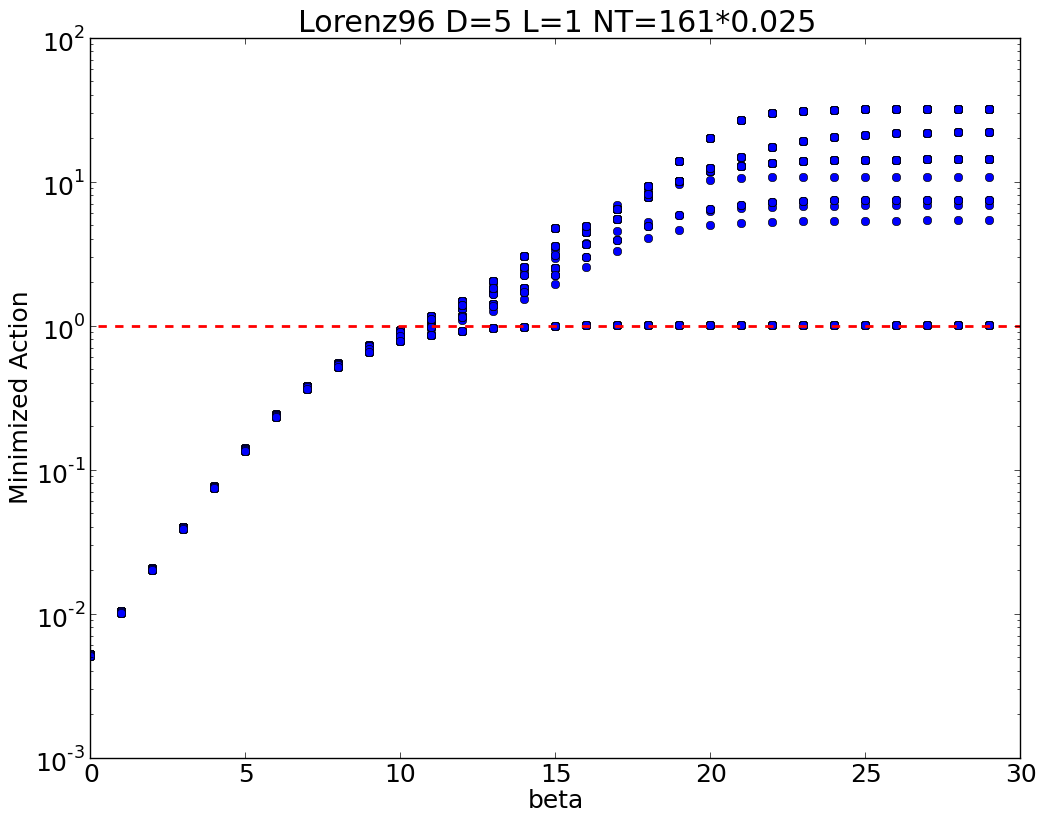
\includegraphics[width=0.8\textwidth]{figure/lorenz96.png}
\caption{Lorenz 96 D=5 L=1 Action Level}
\label{fig:lorenz96}
\end{figure}
\subsection{NaKL}
\paragraph{NaKL Vector Field}
\begin{align*}
\frac{dV}{dt}&=CI_{inj}(t) + g_{Na}m^3h(E_{Na}-V) + g_{K}n^4(E_K-V) + g_L(E_L-V)\\
\frac{da}{dt}&=\frac{a_\infty-a}{\tau_a}, ~~~~a=\{m, h, n\}\\
a_\infty&=\frac12+\frac12\tanh\left(\frac{V-V_a}{\Delta V_a}\right)\\
\tau_a&=\tau_{a0}+\tau_{a0}\left(1-\tanh^2\left(\frac{V-V_a}{\Delta V_a}\right)\right)
\end{align*}
\paragraph{NaKL equations.txt}
\begin{verbatim}
simple_nakl
# nY,nP,nU,nI,nF,nM
4,19,0,1,0,1
#vector field
gNa*(m0*m0*m0*h0)*(ENa-V0)+gK*n0*n0*n0*n0*(EK-V0)+gL*(EL-V0)+Area*Iinj
(0.5*(1+tanh((V0-Vmo)*dVm)) - m0)/(Cm1+Cm2*(1.0-tanh((V0-Vmo)*dVm)*tanh((V0-Vmo)*dVm)))
(0.5*(1+tanh((V0-Vho)*dVh)) - h0)/(Ch1+Ch2*(1.0-tanh((V0-Vho)*dVh)*tanh((V0-Vho)*dVh)))
(0.5*(1+tanh((V0-Vno)*dVn)) - n0)/(Cn1+Cn2*(1.0-tanh((V0-Vno)*dVn)*tanh((V0-Vno)*dVn)))
#obj function
(VDATA0 - V0)*(VDATA0 - V0)
#states
V0
m0
h0
n0
#parameters
gNa
ENa
gK
EK
gL
EL
Area
Vmo
dVm
Cm1
Cm2
Vho
dVh
Ch1
Ch2
Vno
dVn
Cn1
Cn2
#data names
VDATA0
#stimuli
Iinj
\end{verbatim}
\paragraph{NaKL specs.txt}
\begin{verbatim}
3000
0
0.04
#data
./noise_measured.dat
#stimuli
./current.dat
0
#./allstates.dat
# state bounds and Rf0
-150,70,1e-3
0, 1,1e1
0, 1,1e1
0, 1,1e1
# parameter bounds
#gna
50,200,100,120
#Ena
0,100,50,50
#gki
5,40,30,20
#Ek
-100,-50,-70,-77
#gl
0.1,1,.2,.3
#El
-60,-50,-52,-54
#Area
0.5,1.5,1,0.8
#mv1
-60,-30,-45,-40
#mv2
.01,0.1,.075,0.06667
#cm1
0.05,.25,.15,.1
#cm2
.1,1,.4,.4
#hv1
-70,-40,-50,-60
#hv2
-0.1,-.01,-.05,-.06667
#ch1
.1,5,1.2,1
#ch2
1,15,6,7
#nv1
-70,-40,-52,-55
#nv2
.01,0.1,.03,.03333
#cn1
.1,5,.8,1
#cn2
2,12,5,5
#anneal settings
2,1,30
\end{verbatim}
\begin{figure}[h]
\centering
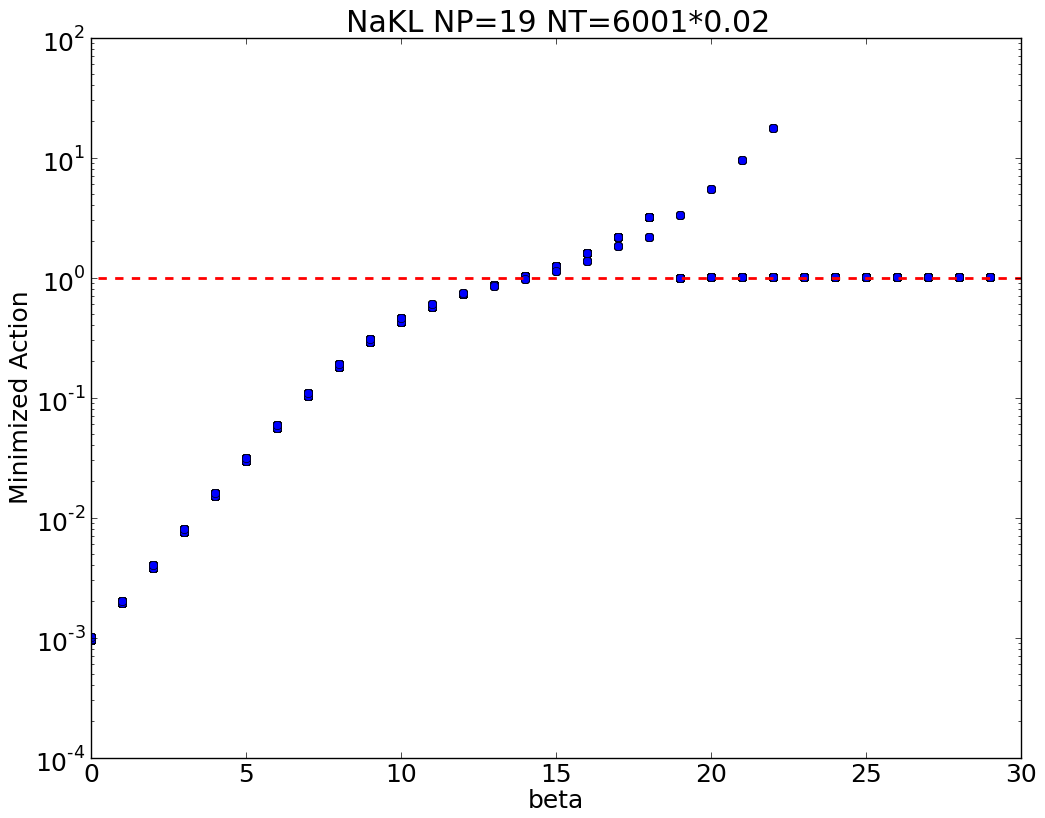
\includegraphics[width=0.8\textwidth]{figure/NaKL.png}
\caption{NaKL Action Level}
\label{fig:NaKL}
\end{figure}
\section{Troubleshooting}
I have tested these scripts over a wide range of problems, so I believe that the algorithms are correct. However, there are a few common errors that may crop up.
\begin{itemize}
\item Variable and parameter naming is very important. At few common problems can crop up. Never use a variable name that includes the name of another variable. For instance p1 and p11 would be bad, since p11 includes p1. In this case, p01 and p11 would be adequate. Along this vein, all variable names should be at least 2 characters long, just in case.
\end{itemize}
\end{document}
